\documentclass{article}
\usepackage[utf8x]{inputenc}
\usepackage{pgfplots}

\begin{document}

\section{Trasarea graficelor pentru funcții explicite}

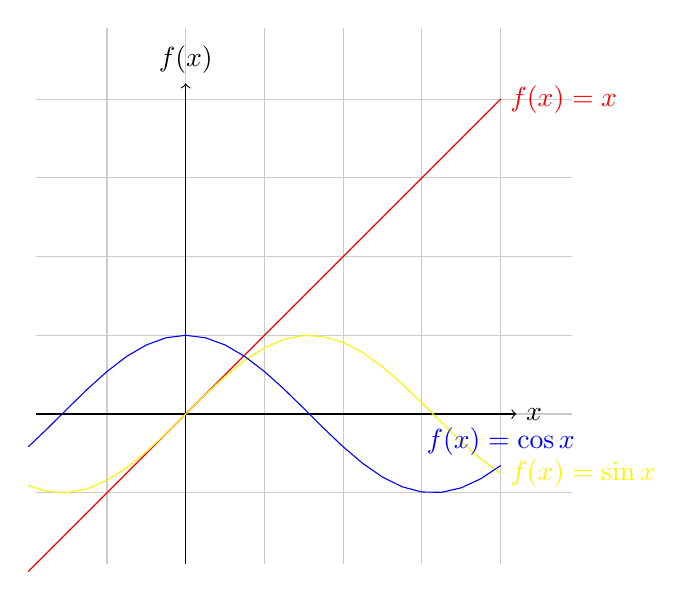
\begin{tikzpicture}[domain=-2:4]
  % grilă
  \draw[help lines,thin,gray!40] (-1.9,-1.9) grid (4.9,4.9);

  % axele
  \draw[->] (-1.9,0) -- (4.2,0) node[right] {$x$};
  \draw[->] (0,-1.9) -- (0,4.2) node[above] {$f(x)$};
  
  % funcții 
  \draw[color=red] plot (\x,\x) node[right] {$f(x) = x$};
  \draw[color=yellow] plot (\x,{sin(\x r)}) node[right] {$f(x) = \sin x$};
  \draw[color=blue] plot (\x,{cos(\x r)}) node[above] {$f(x) = \cos x$};
\end{tikzpicture}

\textbf{1 Exercițiu:} adaugați graficul funcției $x^3$.

\newpage

\section{Trasarea graficelor pentru funcții parametrice}

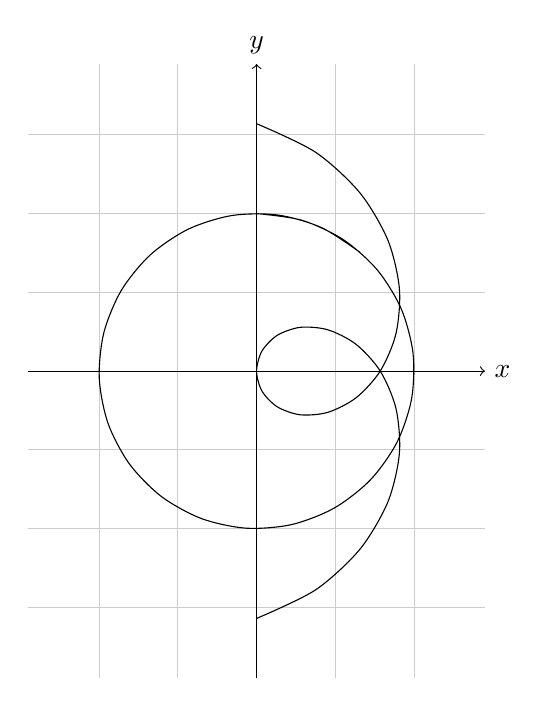
\begin{tikzpicture}
  % grilă
  \draw[help lines,thin,gray!40] (-2.9,-3.9) grid (2.9,3.9);

  % axele
  \draw[->] (-2.9,0) -- (2.9,0) node[right] {$x$};
  \draw[->] (0,-3.9) -- (0,3.9) node[above] {$y$};
  
  % funcții 
  \draw[domain=-3.141:3.141,smooth,variable=\t] plot ({\t*sin(\t r)},{\t*cos(\t r)});
  \draw[domain=0:7, smooth,variable=\t] plot ({2*sin(\t r)},{2*cos(\t r)}); 
\end{tikzpicture}

\newpage

\section{Evaluarea coordonatelor}

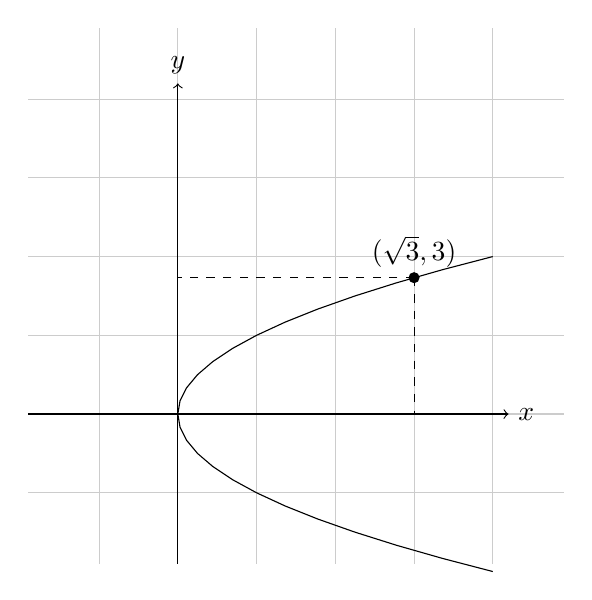
\begin{tikzpicture}[domain=-2:2]
  % grilă
  \draw[help lines,thin,gray!40] (-1.9,-1.9) grid (4.9,4.9);

  % axele
  \draw[->] (-1.9,0) -- (4.2,0) node[right] {$x$};
  \draw[->] (0,-1.9) -- (0,4.2) node[above] {$y$};
  
  % funcții 
  \draw[variable=\y] plot ({(\y)^2},{\y});
  
  \coordinate (P) at (3, {sqrt(3)});
  \fill (P) circle (2pt) node[above] {$(\sqrt{3},3)$};
  
  % proiecțiile
  \draw[dashed] (P) -- (3,0) (P) -- (0,{sqrt(3)});
\end{tikzpicture}


\end{document}